\Chapter{EXTRACTION DE TAXONOMIE}
\label{chap:te}

introduction et présentation générale \ldots


\section{Exposé du problème}
\subsection{Problème}
\label{sec:te-problem}
Soit $\KG \subseteq \Ent \times \Rel \times \Ent$ un graphe de connaissance. Pour une entité $e \in \Ent$, on dit que $e$ est de type $t$ si le triplet $(e, \texttt{rdf:type}, t)$ appartient à $\KG$. Dans la littérature, les types sont souvent appelés des \textit{classes} : ici, on préfère l'usage de \textit{type} pour éviter des conflits de notation avec les \textit{clusters}, qui seront introduits dans la section~\ref{subsec:te-clustering}. Notons qu'une entité peut avoir plusieurs types : ainsi, \dbr{Charles\_Baudelaire} est à la fois de type \dbo{Poet}, \dbo{Writer} et \dbo{Agent}.

On note $\cal{T}$ l'ensemble des types contenus dans le graphe. L'enjeu est de construire une taxonomie $T$ sur $\cal{T}$, c'est-à-dire un ensemble d'axiomes de subsumption $\{(t_i \sqsubseteq t_i')\}_{i=1, \ldots}$. Dans un axiome $t \sqsubseteq t'$, $t$ est appelé un \textit{sous-type} de $t'$, et $t'$ un \textit{supertype} de $t$; l'axiome signifie que $t'$ est un type plus général que $t$, et donc que tout élément de type $t$ est aussi de type $t'$. Pour être valide, une taxonomie $T$ doit vérifier une structure d'arbre, c'est-à-dire respecter deux conditions : chaque type doit avoir au plus un supertype, et $T$ ne doit pas contenir de cycle, donc ne doit contenir aucune séquence $t_0, t_1, \ldots, t_k$ telle que $t_0 \sqsubseteq t_1 \sqsubseteq \ldots \sqsubseteq t_k \sqsubseteq t_0$.

Comme données d'entraînement, on suppose avoir accès à un jeu de données $\cal{D} = \{ (\mathbf{e_i}, t_i) \}_{i=1, \ldots, N}$, constitué de $N$ paires $(\bf{e_i}, t_i) \in \R^d \times \cal{T}$ où $\bf{e_i}$ représente le plongement vectoriel de l'entité $e_i$, et $t_i$ son type. 

Pourquoi ?
extraire l'information taxonomique contenue dans la géométrie des plongements vectoriels
éviter d'exploiter des co-occurrences présentes dans les données, qui peuvent être causées par le fait que l'on a eu accès à une taxonomie lors de la création du graphe.

Relâcher cette contrainte : donne accès au graphe complet, et pas seulement aux embeddings + avoir accès aux co-occurences. Dans ce cas, beaucoup plus d'information = donne la possibilité d'extraire une taxonomie plus riche, cf chapitre suivant.

\subsection{Données}
\label{sec:te-data}

L'ontologie DBpédia comporte un ensemble de classes et de sous-classes qui forment un arbre dont on peu trouver le détail à l'adresse \href{http://mappings.dbpedia.org/server/ontology/classes/}{http://mappings.dbpedia.org/server/ontology/classes/}. Comme on peut le voir, toutes les classes héritent d'une seule classe racine \texttt{owl:Thing} (classe de niveau 0); la profondeur maximale d'une sous-classe est 6. On peut difficilement utiliser toute l'ontologie pour le clustering, car certaines classes très spécifiques contiennent trop peu d'éléments [par exemple, seulement 7 éléments sont de type \texttt{dbo:Star}). On cherche donc à extraire un sous-arbre qui soit (a) suffisamment profond pour modéliser une base de connaissance du monde réel et tel que (b) chaque classe contienne un nombre minimal d'éléments. 

Pour cela, on fixe la profondeur maximale à $p_\max=3$, le nombre maximal de sous-classe par classe à $n_c=7$ et le nombre minimal d'éléments par classe à $n_e=500$. En partant de la classe racine \texttt{owl:Thing}, on ajoute récursivement les sous-classes $S$ d'une classe $C$, par ordre décroissant d'effectif (on commence par ajouter les sous-classes qui contiennent le plus d'éléments), à condition que : 
\begin{itemize}
    \item $S$ contienne au moins $n_e$ entités
    \item la profondeur de $S$ soit au plus $p_\max$
    \item $C$ ait moins de $n_c$ sous-classes
\end{itemize}

Le détail de la taxonomie restreinte ainsi obtenue est présenté en annexe \todo{Ajouter la référence en annexe}. Elle contient 7 classes de niveau 1, qui sont `Agent`, `Event`, `MeanOfTransportation`, `Place`, `Species`, `SportsSeason`, `Work`, 25 classes de niveau 2, et 52 classes de niveau 3. 

J'appelle classes feuilles les classes qui n'ont pas de sous-classes, c'est-à-dire qu'elles sont les plus spécifiques pour qualifier une entité. Les classes feuilles peuvent être de niveau 2, comme par exemple `MeanOfTransportation/Aircraft` ou  `Work/TelevisionEpisode`, mais la plupart sont de niveau 3 (`Agent/Person/Artist` ou `Work/WrittenWork/Comic`). Au total, il y a 64 classes feuilles distinctes.

À partir de cette taxonomie, on tire pour chaque classe feuille un ensemble d'instances DBpédia qui y appartienne. On obtient alors $N=51 418$  instances. Chaque instance est représentée par son plongement, de dimension $d=50$. Le jeu de données consiste donc en une matrice réelle de dimension $51 418 \times 50$.

\section{Méthode proposée}
\label{sec:te-method}
Le préalable à notre méthode est le plongement du graphe dans $\R^d$. Pour cela, on s'appuie sur les travaux préliminaires décrits dans la section~\ref{chap:kge}.
Notre point de départ est donc une matrice de dimension $N \times d$, qui peut être vue comme un nuage de points dans $\R^d$.

\subsection{Regroupement hiérarchique}
\label{subsec:te-clustering}
La première étape consiste à exécuter un algorithme de regroupement (ou \textit{clustering}) hiérarchique agglomératif sur ce nuage de points. 
On commence avec $N$ clusters singletons, chacun contenant l'une des $N$ entités de départ. À chaque étape, deux des clusters existants sont fusionnés pour former un nouveau cluster. Les clusters à fusionner sont choisis de sorte à minimiser un certain critère : ce critère peut être la distance moyenne entre les entités des clusters, la distance minimale ou maximale entre ces entités, ou la variance du nouveau cluster. 
L'algorithme s'arrête lorsqu'il ne reste plus qu'un seul cluster qui contient toutes les entités; ce cluster est appelé cluster racine. Le résultat de cet algorithme est un arbre binaire, dont la racine est le cluster racine contenant toutes les entités, et dont les feuilles sont les $N$ clusters singletons.


On note $\Clusters$ l'ensemble des clusters, $X$ l'arbre de clustering obtenu, et $\texttt{racine}$ la racine de l'arbre – c'est-à-dire, le cluster contenant toutes les entités. On peut écrire $X = (V_X, E_X)$, avec $V_X = \Clusters$ l'ensemble des sommets de $X$, et $E_X = \{(C_i, C_i')\}_{i = 1, 2, \ldots } \subseteq \Clusters^2$ l'ensemble des arêtes de $X$.

Pour deux clusters $C$ et $C'$, on dit que $C$ est un prédecesseur de $C'$ si $C$ appartient à l'unique chemin entre la racine et $C'$, et on note $C \preceq C'$. Dans ce cas, on appelle $C'$ un successeur de $C$, noté $C' \succeq C$. De plus, on dit que $C$ est un prédecesseur \textit{strict} de $C'$ si $C$ est un prédecesseur de $C'$ avec $C \neq C'$. La relation $\prec$ définit un ordre partiel sur l'arbre $X$.

Pour un cluster $C$ donné, on définit $X[C]$ le sous-arbre de racine $C$ comme l'arbre contenant $C$ et tous ses successeurs:
\begin{equation}
    X[C] = (\{C' \in \Clusters : C' \succeq C\}, \{(C_1, C_2) \in E_X : C_2 \succ C_1 \succeq C\})
\end{equation}

Enfin, on définit $\gauche(C)$ et $\droite(C)$ respectivement les sous-clusters gauche et droit de $C$, et $\succs(C)$ l'ensemble des successeurs de $C$.


Considérations temportelles ? Complexité de l'algorithme ?

Étape non-supervisée


\subsection{Association type-cluster}
\label{subsec:te-mapping}

On a d'un côté, une hiérarchie sur des groupes d'entités (les clusters), de l'autre, une liste de types non hiérarchisé; but de l'étape : fusionner ces deux sources d'information, utiliser la structure sur les entités pour créer une structure sur les types. Pour cela, on injecte les types dans l'arbre de clustering, en associant chaque type à un cluster. Pour ce faire, deux méthdoes : 
- associer à chaque type un unique cluster
- définir, pour chaque type, une probabilité d'injection, ou un score d'association avec tous les clusters


\subsubsection{Méthode 1: \textit{Hard Mapping}}
\label{ssubsec:te-hardmapping}

Pour pouvoir associer les types aux clusters pertinents, il faut mesurer à quel point un cluster $C$ donné représente un type $t$. Pour ce faire, on peut utiliser la précision et le rappel de ce cluster pour $t$. Posons $N_{C,t} = | e \in C, type(e) = t|$ le nombre d'entités de type $t$ contenues dans le cluster $C$,
$N_t = |e \in \mathcal{D}, type(e) = t|$ le nombre d'entités de type $t$ dans l'ensemble des données, et $N_C = | C |$ le nombre total d'entitésd dans le cluster $C$. On peut alors définir la précision, le rappel et la mesure $F_1$ :
\begin{align}
    p(C, t) &= \frac{N_{C, t}}{N_C} \\
    r(C, t) &= \frac{N_{C, t}}{N_t} \\
    F(C, t) &= 2 \cdot \frac{p(C, t)r(C, t)}{p(C, t) + r(C, t)} = 2 \cdot \frac{N_{C,t}}{N_C + N_t}
\end{align}

La mesure $F_1$ varie entre 0 et 1: 0 indique que le cluster $C$ ne contient aucune entité de type $t$; 1 signifie que le cluster contient uniquement des entités de type $t$ et que toutes les entités de type $t$ sont contenues dans le cluster. 

Ideally, we would map type $t$ to the cluster that maximizes its F-score, \textit{i.e} choose $m^*(t) = \argmax_C F(C, t)$, but then we could have two types mapped to the same cluster. 
If two types $t_A$ and $t_B$ are mapped to the same cluster $C$, then any type that is mapped to a successor of $C$ will have both $t_A$ and $t_B$ as ancestors, and the resulting taxonomy will not be valid. The mapping thus need to be unambiguous. Formally, this condition means that we need to find a injective mapping between types and clusters $m^* : \mathcal{T} \rightarrow \mathcal{C}$, so that distinct types are mapped to distinct clusters.  

Idéalement, on souhaiterait associer chaque type $t$ au cluster qui maximise sa mesure $F_1$, et donc choisir $m^*(t) = \argmax_C F(C, t)$, mais on pourrait alors avoir deux types associés au même cluster. Or, si deux types $t_A$ et $t_B$ sont associés au même cluster $C$, alors tout type associé à un successeur de $C$ aurait à la fois $t_A$ et $t_B$ comme prédecesseurs, et la taxonomie résultante serait donc invalide, selon les conditions énoncées en section~\ref{sec:te-problem}. Il faut donc garantir une association univoque entre types et clusters. Formellement, cela signifie que la fonction d'association $m^* : \Types \rightarrow \Clusters$ entre les types et les clusters doit être injective :
\begin{equation}
    \forall t, t' \in \Types, t \neq t' \implies m^*(t) \neq m^*(t')
\end{equation}


Pour une injection $m : \Types \rightarrow \Clusters$, on définit un score $J(m)$ qui mesure la qualité de l'association type-cluster définie par $m$. Ce score est simplement la mesure $F_1$ globale induite par $m$ :
\begin{equation}
    J(m) = \sum_{t \in \mathcal{T}} F(m(t), t)
\end{equation}

Notre association optimale est alors :
\begin{equation}
    m^* = \argmax_{
\substack{m : \Types \rightarrow \Clusters \\ m\text{ injective}}} \sum_{t \in \mathcal{T}} F(m(t), t)
\label{eq:optim-mapping}
\end{equation}


L'équation~\ref{eq:optim-mapping} définit un problème d'affectation linéaire, pour lequel une solution optimale existe dans tous les cas (et est unique si les mesures $F_1$ sont uniques pour chaque cluster).
Cette solution optimal peut être trouvée par l'algorithme de Jonker-Volgenant, avec une complexité de $O(|\Clusters|^3)$ dans le pire des cas \cite{jonker1987shortest}. Toutefois, l'utilisation de l'heuristique \textit{Asymmetric Greedy Search} \cite{brown2017heuristic} permet de réduire cette complexité, tout en trouvant des solutions dont le score est supérieur à 99.9\% du score optimal, en moyenne.
%, which can be useful when the size of $\mathcal{D}$ increases.

\subsubsection{Méthode 2: \textit{Soft Mapping}}
\label{ssubsec:te-softmapping}

L'approche précédente aboutit à une fonction de décision binaire : un axiome $(t_i \sqsubset t_j)$ est prédit ou non, sans intermédiaire possible. Ceci parce que la fonction $\argmax$ de l'équation~\ref{eq:optim-mapping} n'est pas continue. En conséquence, la taxonomie prédite est sensible à des légers changements dans les données d'entrée.

Dans cette version, on explore une version lissée de l'approche précédente : l'association entre types et clusters est conservée, mais elle est lissée en remplacant la fonction $\argmax$ par une fonction softmax. Ainsi, un type n'est plus associé à un unique cluster; on lui attribue plutôt un vecteur de probabilité qui mesure combien chaque cluster le répresente bien. Ensuite, comme précédemment, cette association type-cluster est utilisée pour transformer la hiérarchie des clusters en une hiérarchie des types. Par rapport au cas précédent, la condition d'injectivité de l'association disparaît : une étape supplémentaire est nécessaire pour transformer le graphe de subsumption en une taxonomie valide. Ainsi, la discontinuité identifiée précédemment ne disparaît pas, mais elle est déplacée : au lieu d'intervenir lors de l'extraction des axiomes de subsumption, elle apparaît lors de la création de la taxonomie prédite à partir de ces axiomes. 

La première étape est de transformer les mesures $F_1$ en probabilités, à l'aide d'une fonction softmax. Pour un type $t$ et un cluster $C$, on définit ainsi la probabilité que le cluster $C$ représente le type $t$ :
\begin{equation}
    P(m(t) = C) = \frac{\displaystyle e^{ \beta F(t, C)}}{\displaystyle \sum_{C' \in \mathcal{C}} e^{\beta F(t, C')}}
\end{equation}

Le paramètre $\beta > 0$ contrôle la concentration de la distribution autour du maximum. Le cas $\beta \rightarrow 0$ attribue à tous les axiomes la même probabilité, tandis que le cas $\beta \rightarrow \infty$ donne toute la masse de probabilité à la valeur maximum, ce qui se rapproche de l'approche précédente. Le choix de la valeur de $\beta$ est discuté dans la section 

Ce score d'injection $P(m(t) = C)$ peut ensuite être utilisé pour calculer la probabilité d'un axiome de subsumption $(t' \sqsubset t)$, en tirant profit de la structure d'arbre qui existe entre les clusters. 
Écrire ce score d'injection comme une probabilité $P(m(t) = C)$ permet d'interpréter $(m(t) = C)$ comme un événement aléatoire, et donc $m(t)$ comme une variable aléatoire. On peut donc envisager l'approche de la façon suivante : le type $t$ est localisé quelque part dans l'arbre de clustering, mais cette localisation est entachée d'incertitude, ce que modélise la variable aléatoire $m(t)$. Par définition du softmax, la position la plus probable de $t$ est le cluster qui a le score $F_1$ le plus élevé; toutefois, là où la méthode du hard mapping ne considérait pas d'autre possibilité, d'autres positions de $t$ sont possibles. 

Dès lors, l'axiome $(t' \sqsubset t)$ est lui aussi un événément aléatoire. Cet événement se réalise si, dans l'arbre, \ldots

Note : une idée : et si on notais $Z_t$ la variable aléatoire correspondant à $m(t)$ ? Ça simplifierais peut etre les notations et la compréhension de la méthode. $m(t)$ c'est pas clair ce que ça représente, alors que $Z_t$ ça représente le cluster associé à $t$ (comme dans le hard mapping), sauf qu'on ne sait pas ù est $Z_t$. Intro : «on modélise la situation> (comme c'est une modélisation on est plus comptables de la véracité de nos hypothèses, notamment l'indepndance des $Z_t$)

On définit un score d'association $\sigma(t, C)$:
\begin{equation}
    \sigma(t, C) = \frac{\displaystyle e^{ \beta F(t, C)}}{\displaystyle \sum_{C' \in \mathcal{C}} e^{\beta F(t, C')}}
\end{equation}

On définit une famille de variables aléatoire $\cal{Z} = (Z_t)_{t \in \Types}$, indépendantes et à valeur dans $\Clusters$. Pour un type $t$ donné, la loi de la variable $Z_t$ est donné par :
\begin{equation}
    P(Z_t = C) = \sigma(t, C)
\end{equation}
On interprète la variable aléatoire $Z_t$ comme le cluster associé à $t$ dans l'arbre de clustering. Contrairement au cas précédent, où on aurait eu $Z_t = \argmax_C F(C, t)$ (à la condition d'injectivité près), ici on accepte que l'associé de $t$ soit incertain. \todo{Justifier l'indépendance}

Dès lors, on peut interpréter l'événement $t' \sqsubset t$ comme l'événement $Z_t \prec Z_{t'}$, et donc, en utilisant l'indépendances des $Z_t$ : 
\begin{align}
    \label{eq:softmapping_2}
    P(t' \sqsubset t) &= P(Z_t \prec Z_{t'}) \\
    &= \sum_{\substack{C_A, C_B \in \mathcal{C} \\ C_A \prec C_B}} P(Z_{t }= C_A, Z_{t'} = C_B) \nonumber \\
    &= \sum_{\substack{C_A, C_B \in \mathcal{C} \\ C_A \prec C_B}} P(Z_{t }= C_A)\cdot P(Z_{t'} = C_B)
\end{align}

Pour calculer ces probabilités pour chaque $t, t'$ sans sommer sur toutes les paires de clusters, on peut concevoir un algorithme récursif de type «diviser pour régner». Pour cela, il nous faut exprimer $P(t' \sqsubset t)$ sous forme récursive. On introduit donc une nouvelle quantité,  $P_C(t' \sqsubset t)$ : c'est, comme dans l'équation~\ref{eq:softmapping_2}, la probabilité de l'événement $t' \sqsubset t$ (c'est-à-dire de l'événément $Z_t \prec Z_{t'}$), mais restreint au cas où $Z_t$ et $Z_{t'}$ appartienent au sous-arbre $X[C]$. Or appartenir au sous-arbre $X[C]$ est équivalent à être un successeur de $C$, on peut donc réécrire l'événement $(Z_t \prec Z_{t'}) \land (Z_t, Z_{t'} \in X[C])$ sous la forme $C \preceq Z_t \prec Z_{t'}$. D'où :
\begin{align}
    P_C(t' \sqsubset t) &= P(C \preceq Z_t \prec Z_{t'}) \nonumber \\
    &= \sum_{\substack{C_A, C_B \in \succs(C) \\  C_A \prec C_B}} P(Z_t = C_A)\cdot P(Z_{t'} = C_B) \label{eq:proba_subsumption}
\end{align}


% To compute these probabilities for all $t, t'$ without summing over all pairs of % clusters, we devise a divide-and-conquer algorithm. For this, we need a recursive % formulation of $P(t' \sqsubset t)$, so we introduce $P_C(t' \sqsubset t)$, the % probability of axiom $(t' \sqsubset t)$ computed on the subtree $X[C]$, for any given % cluster $C$. Similarly to equation~\ref{eq:softmapping_2}, it represents the % probability that the cluster $m(t)$ representing $t$ is a predecessor of  the cluster % $m(t')$ representing $t'$, with the additional condition that both $m(t)$ and $m(t')$ % must belong to the subtree $X[C]$ (that is, be successors of $C$):
% \begin{align}
%     P_C(t' \sqsubset t) &= P(C \preceq m(t) \prec m(t') % \text{ and } m(t),m(t') % \succeq C %, C \preceq m(t')
%     ) \nonumber \\
%     &= \sum_{\substack{C_A, C_B \in \succs(C) \\ C_A \prec C_B}} P(m(t) = C_A)\cdot % P(m(t') = C_B) 
%     \label{eq:proba_subsumption}
% \end{align}

Comme le sous-arbre $X[\texttt{racine}]$ est égal à l'arbre complet, on a $P_\texttt{racine}(t' \sqsubset t) = P(t' \sqsubset)$. Si on parvient à exprimer $P_\texttt{racine}$ en fonction de $P_{\gauche(\texttt{racine})}$ et de $P_{\gauche(\texttt{racine})}$

\ldots 

Soit $L = \gauche(C)$ et $R = \droite(C)$ les sous-clusters gauche et droit de $C$. On peut remarquer qu'un successeur de $C$ est soit un successeur de $L$, soit un successeur de $R$, soit $C$ lui-même. Autrement dit, en notant $\sqcup$ l'union disjointe :
\begin{equation}
    \succs(C) = \succs(L) \sqcup \succs(R) \sqcup \{ C\}
\end{equation}
En suivant cette observation, on peut donc partager la somme~\ref{eq:proba_subsumption} en trois :
\begin{align}
P_{C}(t' \sqsubset t) = 
&
\sum_{\substack{C_A, C_B \in \succs(L) \\  C_A \prec C_B}} P(Z_t = C_A)\cdot P(Z_{t'} = C_B) 
\nonumber \\ 
&+ 
\sum_{\substack{C_A, C_B \in \succs(R) \\  C_A \prec C_B}} P(Z_t = C_A)\cdot P(Z_{t'} = C_B) 
\nonumber \\
&+ \displaystyle \sum_{C_B \colon C \prec C_B} P(Z_t = C) \cdot P(Z_{t'} = C_B) \nonumber \\
= {} & P_{L}(t' \sqsubset t) + P_{R}(t' \sqsubset t)  + P(Z_t=C)\cdot\sum_{\substack{C_B \colon \\ C\prec C_B}} P(Z_{t'} = C_B)
\label{eq:proba_over_subtree}
\end{align}

Cette équation fait apparaître le lien recherché entre $P_C$ d'un côté, et $P_L$ et $P_R$ de l'autre. On l'écrire de façon plus concise sous forme matricielle. Pour cela, définissons $n_T = | \mathcal{T} |$ le nombre de types distincts, $\mathbf{Q_C}$ une matrice de dimension $n_T \times n_T$ telle que sa coordonnée $(i, j)$ contienne $P_C(t_j \sqsubset t_i)$, et $\mathbf{p_C} = \left(P(Z_{t_i} = C)\right)_{i = 1, \ldots, n_T}$ le vecteur de probabilité du cluster $C$, de dimension $n_T$. 

Avec ces notations, notre objectif est de calculer $\bf{Q_\texttt{racine}}$, et donc d'obtenir une formule récursive reliant $\bf{Q_C}$ à $\bf{Q_L}$ et $\bf{Q_R}$. L'équation \ref{eq:proba_over_subtree} se réécrit :
\begin{align}
    \mathbf{Q_C} &= \mathbf{Q_L} + \mathbf{Q_R} + \mathbf{p_C} \cdot \left(\sum_{C' \colon C \prec C'} \mathbf{p_{C'}} \right)^\top 
    \label{eq:recursive_q_formula}
\end{align}

À ce stade, l'équation \ref{eq:recursive_q_formula} est proche de la formulation récursive cherchée, mais il reste encore à éliminer la somme $\sum_{C' \colon C \prec C'} \mathbf{p_{C'}}$, parce qu'elle dépend de tous les successeurs stricts de $C$, et pas seulement de $C, L$ ou $R$. On note donc $\bf{s_C}$ cette somme :
\begin{align}
    \bf{s_C} &= \sum_{C' \colon C \prec C'} \mathbf{p_{C'}} \nonumber \\
            &= \sum_{C' \in \succs(C)^*} \mathbf{p_{C'}}
\end{align}
Cette somme est un vecteur de dimension $n_T$; sa $i$-ème coordonnée représente la probabilité pour le type $t_i$ d'être associé à un successeur strict de $C$, c'est-à-dire $P(Z_{t_i} \succ C)$. Or un successeur strict de $C$ est soit $L$ ou $R$, soit un successeur strict de $L$ ou $R$, ce qui s'exprime mathématiquement par :
\begin{equation}
    \succs(C)^* = \{L\} \sqcup \{R\} \sqcup \succs(L)^* \sqcup \succs(R)^*
\end{equation}

On peut donc réécrire $\bf{s_C}$ comme :
\begin{align}
    \mathbf{s_C} &= \mathbf{p_L} + \mathbf{p_R} + (\mathbf{s_L} + \mathbf{s_R}) \nonumber  \\
     &= (\mathbf{p_L}  + (\mathbf{s_L}) + (\mathbf{p_R} + \mathbf{s_R})
    \label{eq:l_def}
\end{align}
Finalement, on définit la probabilité pour chaque type d'être associé à un successeur non-strict de $C$ : 
\begin{equation}
    \mathbf{u_C} = \mathbf{p_C} + \mathbf{s_C}
    \label{eq:def_uc}
\end{equation}
Cela permet de reformuler ainsi l'équation \ref{eq:l_def}:
\begin{equation}
    \mathbf{s_C} = \mathbf{u_L} + \mathbf{u_R}
    \label{eq:l_update}
\end{equation}

On a désormais nos équations de récurrences : \ref{eq:recursive_q_formula} pour $\bf{Q_C}$, \ref{eq:def_uc} pour $\bf{u_C}$ et \ref{eq:l_update} pour $\bf{s_C}$. Il reste à calculer les cas de base, c'est-à-dire les valeurs de $\bf{Q, u, s}$ pour les clusters feuilles. Si $C$ est une feuille, la probabilité pour un type $t$ d'être associé à un de ses successeurs stricts est nulle, puisque $C$ n'a aucun successeur strict. Pour la même raison, la probabilité pour qu'un axiome de subsumption $t' \sqsubset t$ soit vérifié dans le sous-arbre $X[C]$ est également zéro. Ainsi $\mathbf{s_C}$ et $\mathbf{Q_C}$ sont respectivement nuls pour chaque cluster feuille. Quant à $\bf{u_C}$, sa valeur sur les feuilles peut être calculée par l'équation \ref{eq:def_uc}.

On peut finalement écrire les équations de récurrence pour $\mathbf{s_C}, \mathbf{Q_C}, \mathbf{u_C}$:
\begin{align}
    \mathbf{Q_C} &=
    \begin{cases}
      \mathbf{0}_{n_T,n_T} & \text{si $C$ est une feuille}\\
      \mathbf{p_C} \cdot \mathbf{s_C}^\top + \mathbf{Q_\text{left$(C)$}} + \mathbf{Q_\text{right$(C)$}} & \text{sinon}
    \end{cases}  \\
  \mathbf{s_C} &=
    \begin{cases}
      \mathbf{0}_{n_T} & \text{si $C$ est une feuille}\\
      \mathbf{u_\text{left$(C)$}} + \mathbf{u_\text{right$(C)$}} & \text{sinon}
    \end{cases}  \\
    \mathbf{u_C} &= \mathbf{p_C} + \mathbf{s_C}
\end{align}

Our implementation uses linear programming. We denote $D_C = (\mathbf{s_C}, \mathbf{Q_C}, \mathbf{u_C})$. Clusters are iterated over in a reverse DFS order. For each cluster $C$, we compute and cache $D_C$ using $D_{\text{left}(C)}$ and $D_{\text{right}(C)}$. The reverse DFS order guarantees that all successors of $C$ have already been visited, so $D_{\text{left}(C)}$ and $D_{\text{right}(C)}$ are already cached. After computing $D_C$, we can delete cached values $D_{\text{left}(C)}$ and $D_{\text{right}(C)}$ because no further computation depends on them. The last visited cluster is $\texttt{root}$: when the algorithm ends, the cache contains only $D_\texttt{root} = (\mathbf{s_\texttt{root}}, \mathbf{Q_\texttt{root}}, \mathbf{u_\texttt{root}})$, and the final probability matrix $\mathbf{Q_\texttt{root}}$ can be returned. Its $(i, j)$ coordinate contains the probability of axiom $(t_j \sqsubset t_i)$.
For a balanced binary tree, this algorithm guarantees a maximum cache size of $O(|\mathcal{T}|^2 \log_2(| \mathcal{C} |))$, with $|\mathcal{T}| \ll | \mathcal{C} |$.


\subsection{Construction de la taxonomie}
\label{subsec:te-taxconstruction}

\section{Évaluation et discussion}
\label{sec:te-evaluation}

\subsection{Méthode d'évaluation}
\label{subsec:te-evaluation}

\subsection{Résultats}
\label{subsec:te-results}

\begin{table}
    \centering
    \caption{
    Évaluation de notre approche et de TIEmb sur \textsc{DBpedia-Freq}, pour différents modèles de plongement. $p, r, F1$ désignent respectivement la précision, le rappel et la mesure $F1$. \textit{cos} et \textit{euc} indiquent les distances cosinus et euclidienne. Les résultats de la section \textit{Moyenne} sont obtenus en calculant la moyenne des évaluations directe et transitive.}
    \begin{tabular}{|lll|ccc|ccc|ccc|}
    \hline 
                               &      &          & \multicolumn{3}{c|}{Directe}              & \multicolumn{3}{c|}{Transitive}     & \multicolumn{3}{c|}{Moyenne}     \\
        Méthode	&	Plongements	&	Distance	&	$p$	&	$r$	&	$F$	&	$p$	&	$r$	&	$F1$	&	$p$	&	$r$	&	$F1$	\\	
\hline \multirow{8}{*}{TIEmb}	&	\multirow{2}{*}{ComplEx}	&	cos	&	0.38	&	0.38	&	0.38	&	0.28	&	0.57	&	0.37	&	0.33	&	0.48	&	0.38	\\
	&		&	euc	&	0.39	&	0.42	&	0.4	&	0.34	&	0.8	&	0.48	&	0.37	&	0.61	&	0.44	\\[2pt] 
	&	\multirow{2}{*}{DistMult}	&	cos	&	0.26	&	0.27	&	0.26	&	0.19	&	0.44	&	0.27	&	0.23	&	0.36	&	0.27	\\
	&		&	euc	&	0.37	&	0.41	&	0.39	&	0.33	&	0.79	&	0.47	&	0.35	&	0.60	&	0.43	\\[2pt] 
	&	\multirow{2}{*}{RDF2Vec}	&	cos	&	0.77	&	\textbf{0.84}	&	0.81	&	0.43	&	0.87	&	0.57	&	0.60	&	0.86	&	0.69	\\
	&		&	euc	&	0.70	&	0.77	&	0.73	&	0.30	&	0.73	&	0.42	&	0.50	&	0.75	&	0.58	\\[2pt] 
	&	\multirow{2}{*}{TransE}	&	cos	&	0.77	&	0.72	&	0.74	&	0.83	&	0.89	&	0.86	&	0.80	&	0.81	&	0.80	\\
	&		&	euc	&	0.76	&	0.75	&	0.76	&	0.7	&	0.9	&	0.79	&	0.73	&	0.83	&	0.78	\\[2pt] 
\hline \multirow{8}{*}{\shortstack[c]{Hard Mapping \\ (HM)}}	&	\multirow{2}{*}{ComplEx}	&	cos	&	0.53	&	0.5	&	0.52	&	0.78	&	0.7	&	0.74	&	0.66	&	0.60	&	0.63	\\
	&		&	euc	&	0.51	&	0.44	&	0.47	&	0.87	&	0.52	&	0.65	&	0.69	&	0.48	&	0.56	\\[2pt] 
	&	\multirow{2}{*}{DistMult}	&	cos	&	0.55	&	0.47	&	0.5	&	0.73	&	0.57	&	0.64	&	0.64	&	0.52	&	0.57	\\
	&		&	euc	&	0.43	&	0.36	&	0.39	&	0.75	&	0.54	&	0.63	&	0.59	&	0.45	&	0.51	\\[2pt] 
	&	\multirow{2}{*}{RDF2Vec}	&	cos	&	0.60	&	0.44	&	0.50	&	0.88	&	0.50	&	0.63	&	0.74	&	0.47	&	0.57	\\
	&		&	euc	&	0.60	&	0.53	&	0.56	&	0.89	&	0.64	&	0.74	&	0.74	&	0.58	&	0.65	\\[2pt] 
	&	\multirow{2}{*}{TransE}	&	cos	&	0.82	&	0.8	&	0.81	&	0.97	&	0.89	&	\textbf{0.93}	&	\textbf{0.90}	&	0.85	&	0.87	\\
	&		&	euc	&	0.73	&	0.67	&	0.7	&	\textbf{0.99}	&	0.68	&	0.8	&	0.86	&	0.68	&	0.75	\\[2pt] 
\hline \multirow{8}{*}{\shortstack[c]{Soft Mapping \\ (SM)}}	&	\multirow{2}{*}{ComplEx}	&	cos	&	0.52	&	0.48	&	0.5	&	0.89	&	0.7	&	0.79	&	0.71	&	0.59	&	0.65	\\
	&		&	euc	&	0.51	&	0.44	&	0.47	&	0.84	&	0.6	&	0.7	&	0.68	&	0.52	&	0.59	\\[2pt] 
	&	\multirow{2}{*}{DistMult}	&	cos	&	0.5	&	0.44	&	0.47	&	0.87	&	0.65	&	0.74	&	0.69	&	0.55	&	0.61	\\
	&		&	euc	&	0.48	&	0.42	&	0.45	&	0.86	&	0.65	&	0.74	&	0.67	&	0.54	&	0.60	\\[2pt] 
	&	\multirow{2}{*}{TransE}	&	cos	&	\textbf{0.83}	&	0.81	&	\textbf{0.82}	&	0.93	&	\textbf{0.93}	&	\textbf{0.93}	&	0.88	&	\textbf{0.87}	&	\textbf{0.88}	\\
	&		&	euc	&	0.78	&	0.77	&	0.77	&	0.98	&	0.87	&	0.92	&	0.88	&	0.82	&	0.85	\\[2pt] 
\hline
    \end{tabular}
    \label{tab:te-results}
\end{table}


\subsection{Discussion}
\label{subsec:te-discussion}

\section{Hyperparamètres}
\label{sec:te-hp}
\subsection{Base \texorpdfstring{$\beta$}{beta} du softmax}
\label{subsec:te-hp-beta}

\begin{figure}
    \centering
    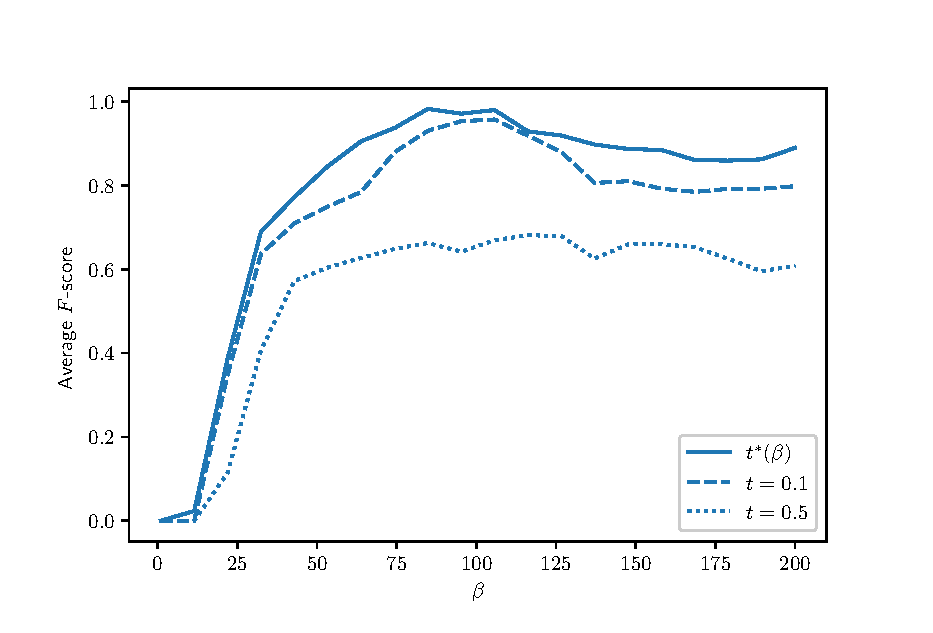
\includegraphics{fig/plot/average_beta_vs_best.eps}
    \caption{Taxonomy extraction $F$-scores obtained for different values of parameter $\beta$, with the optimal threshold $t^*(\beta)$ and two fixed threshold $0.1$ and $0.5$. Scores are averaged over five different subtaxonomies of DBpedia, and expressed as a fraction of the optimal score.}
    \label{fig:beta-search-1}
\end{figure}

\begin{figure}
    \centering
    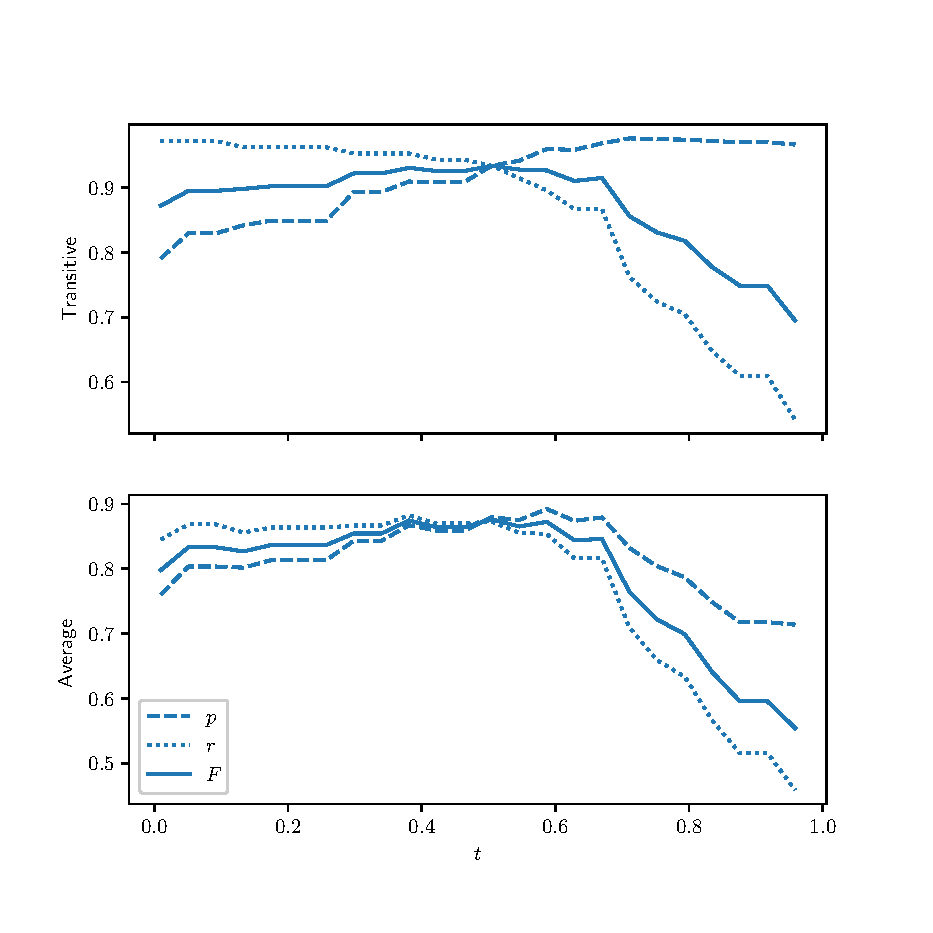
\includegraphics{fig/plot/threshold_exp.eps}
    \caption{Taxonomy extraction $F$-scores obtained for different values of parameter $\beta$, with the optimal threshold $t^*(\beta)$ and two fixed threshold $0.1$ and $0.5$. Scores are averaged over five different subtaxonomies of DBpedia, and expressed as a fraction of the optimal score.}
    \label{fig:beta-search-2}
\end{figure}

\begin{figure}
    \centering
    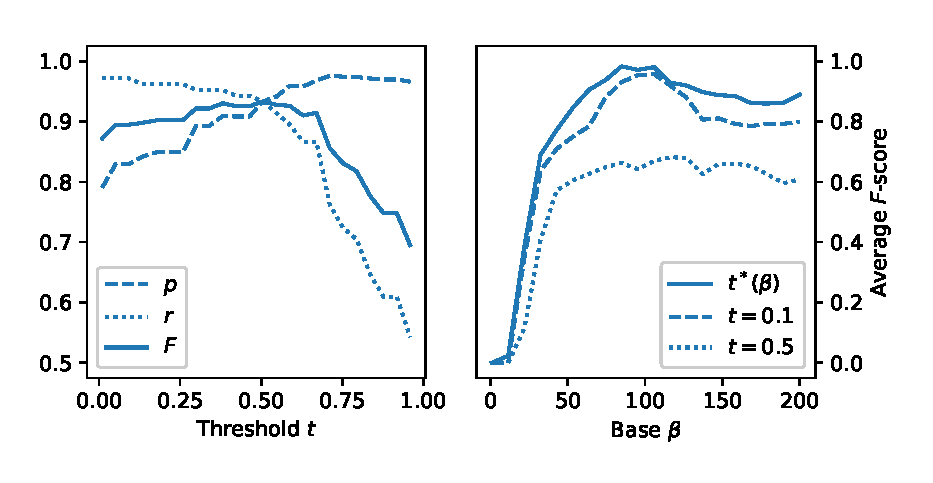
\includegraphics[width=\textwidth]{fig/plot/hp_results.eps}
    \caption{Influence des hyperparamètres $t$ et $\beta$ pour la méthode «soft mapping». À gauche, la précision, rappel et mesure $F1$ obtenus par évaluation transitive pour différentes valeurs de $t$ dans $[0, 1]$, et $\beta = 100$. À droite, les mesures $F1$ obtenues pour différentes valeurs du paramètre $\beta$, et pour trois différents seuils : le seuil optimal $t^*(\beta)$ et deux seuils fixes $t=0,1$ et $t=0,5$. Les scores affichés sont obtenus en moyennant les résultats obtenus sur cinq sous-taxonomies de DBpedia, et exprimées comme une fraction du score optimal.
    }
    \label{fig:t-search-1}
\end{figure}

